\section{Description de la base de données}
\subsection{Schéma entité-association}

\subsection{Schéma relationnel}
Le schéma de la base de données est la figure \ref{fig:bdd} à la page \pageref{fig:bdd}.
Ce schéma a été généré à partir de notre schéma entité-association dans DB-MAIN.

Comme vu dans le schéma entité-association (fig.~\ref{fig:ea} p.\pageref{fig:ea}), les entités \textit{client}, \textit{propriétaires}, \textit{agent} sont des fils de l'entité \textit{personne}. Nous avions donc le choix pour le représentation relationnel entre combiner ces trois entités fils dans une même table ou de les dissocier dans trois tables. Nous avons opté pour la deuxième solution. Il est plus aisé d'avoir les clients et les propriétaires dans des tables distinctes, car ces deux entités ont des attributs différents. Nous avons plus d'informations à conserver pour un client que pour un propriétaire.

\begin{figure}[H]
	\centering
	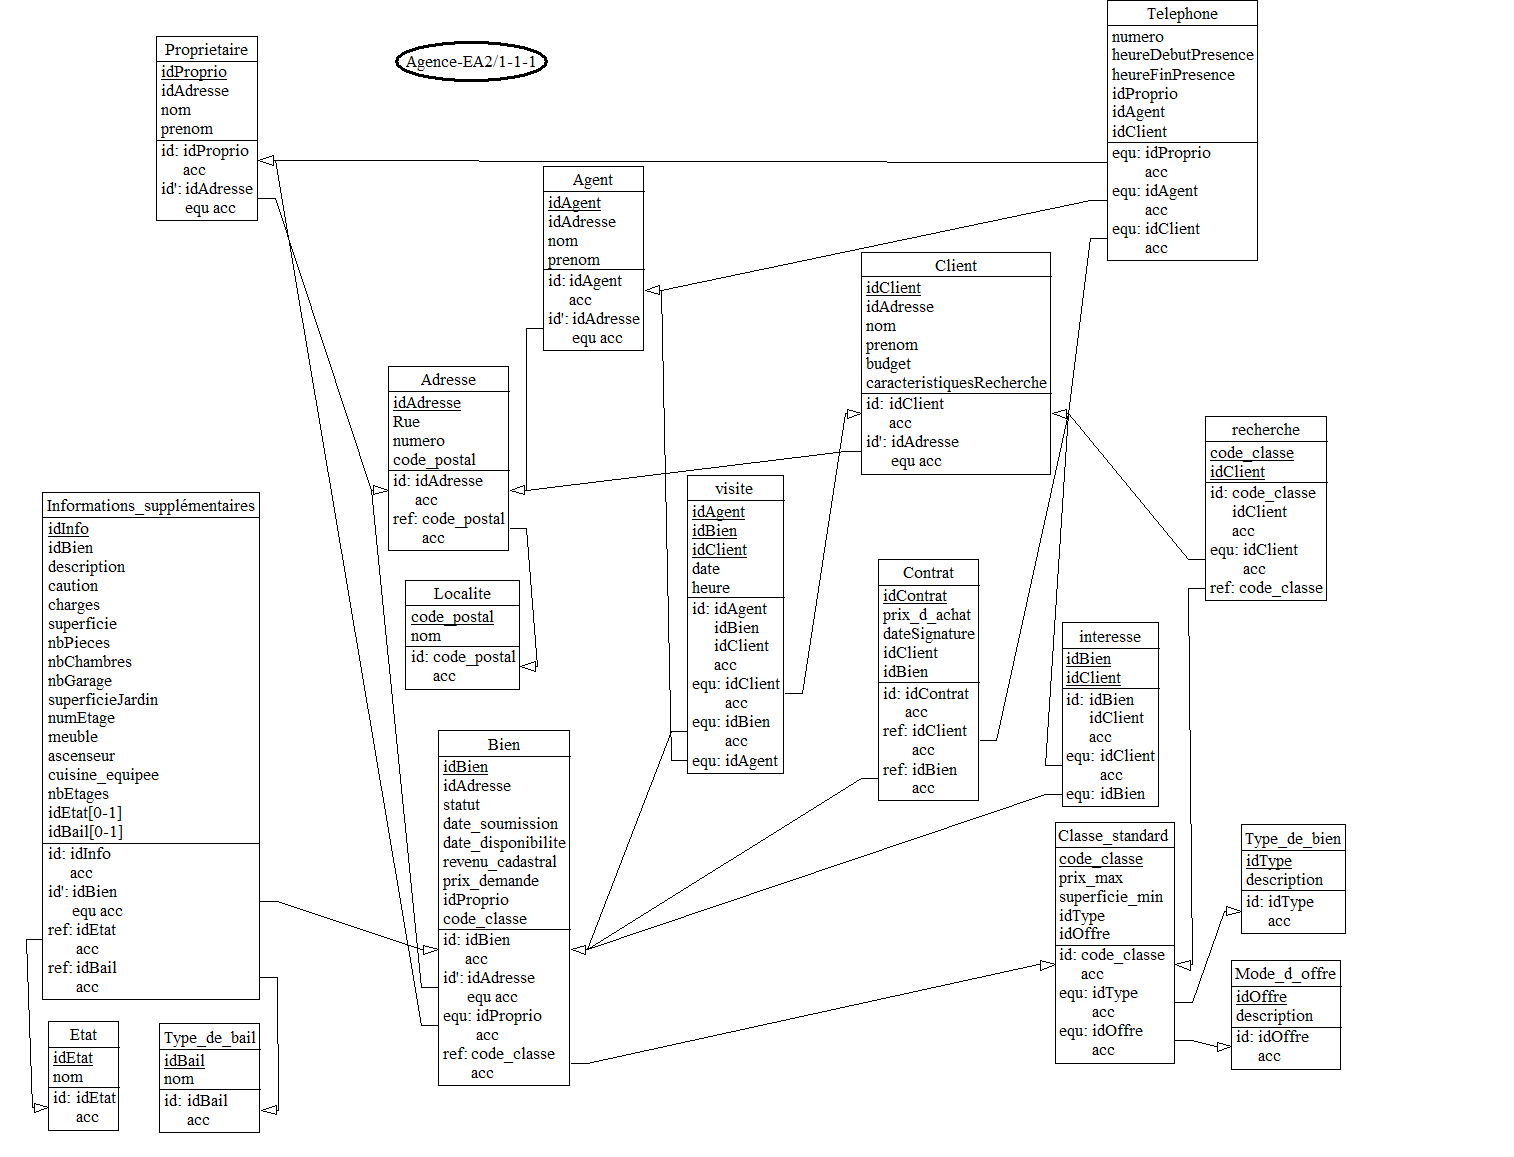
\includegraphics[width=16cm]{relationnel.png}
	\caption{Schéma de la base de données}
	\label{fig:bdd}
\end{figure}

\newpage
\begin{landscape}
	\begin{figure}
		\centering
		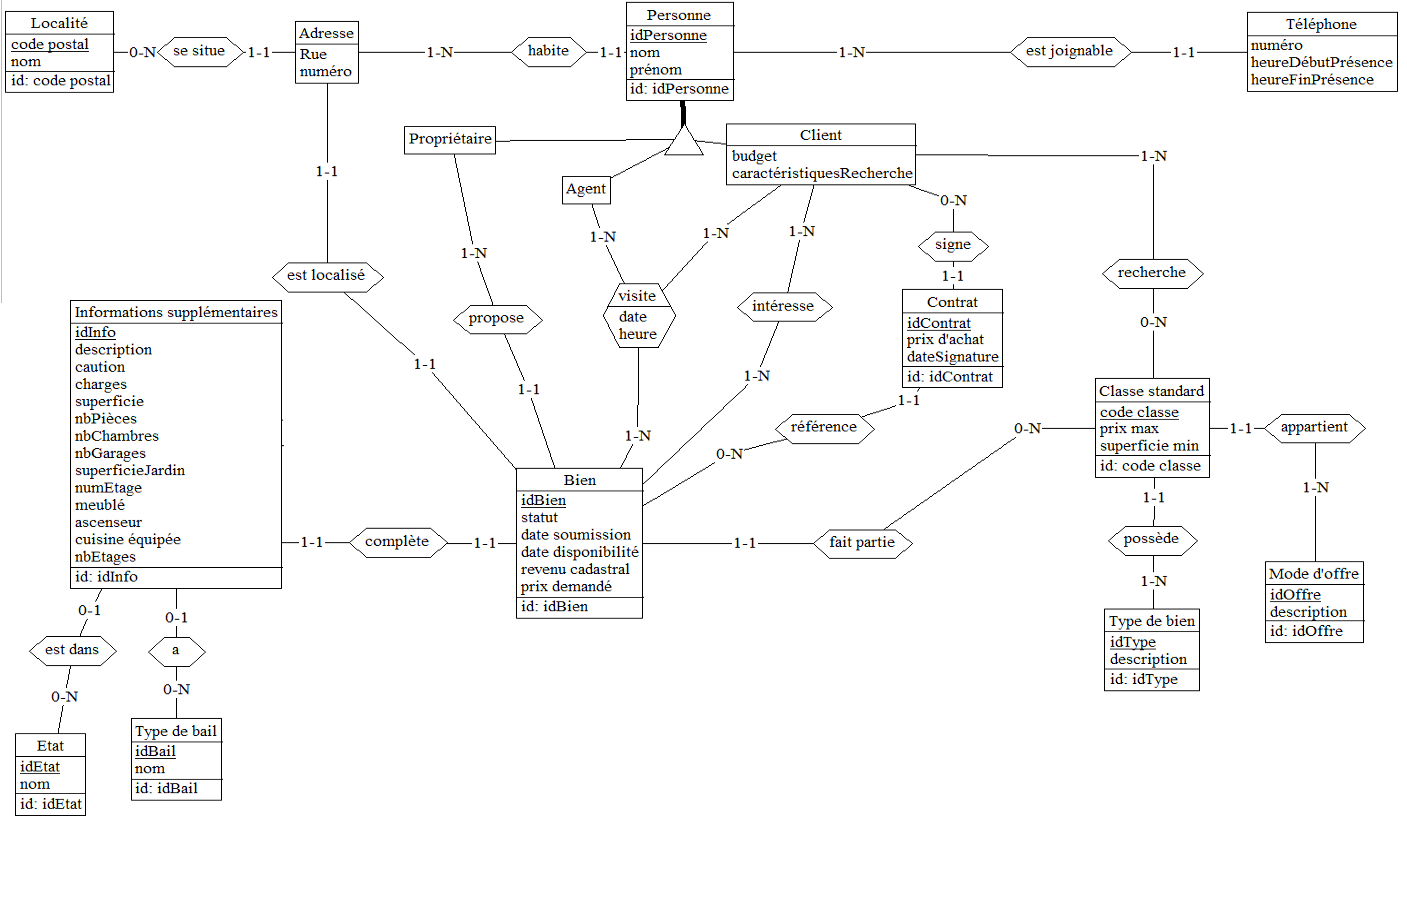
\includegraphics[width=25cm]{association.png}
		\caption{Schéma entité-association final}
		\label{fig:ea}
	\end{figure}
\end{landscape}

